\documentclass[12pt, a4paper]{article}

\usepackage[spanish]{babel}

\usepackage{amsmath} % Escritura mejorada de fórmulas matemáticas
\usepackage{graphicx} % Inserción de gráficos
\usepackage{algorithm}
\usepackage{algpseudocode}

\usepackage[colorlinks=true, citecolor=blue]{hyperref}


\title{Crossword CBD}
\author{Pedro González Marcos}
\date{27 de Mayo 2024}

\begin{document}

\maketitle

\tableofcontents

\section{Introducción}

La idea de este trabajo surge principalmente de una necesidad doble
que tenía antes de los exámenes de la primera convocatoria de CBD.

Hacer el proyecto de CBD y prepararme para el tipo test de la asignatura.

Entonces se me ocurrió implementar una aplicación de crucigrama que
tematizada en la asignatura. 




\section{Cuestiones previas}

Para poner en contexto al que no esté familiarizado con este juego.
El crucigrama es un pasatiempo donde tienes que introducir palabras
en una cuadrícula siguiendo las pistas proporcionadas.

Hay dos tipos de celdas en un cuadrícula las celdas negras o bloques y las
celdas blancas en donde puedes introducir una letra.

Las celdas que empiece una palabra tiene un número. Este número sirve
para hacer referencia a las pistas del crucigrama. 

La gracia del crucigrama es que si no te sabes una pista en horizontal o en 
vertical puedes solucionarlo mirando otras pistas.

\subsection{Convención de crucigrama americano}

Para la implementación del algoritmo que encuentra las palabras dentro del
crucigrama, se han hecho las siguientes suposiciones:

\begin{itemize}
	\item Las palabras están formadas por al menos 3 letras.
	\item El crucigrama debe ser simétrico si lo rotamos 180º, es decir
	imaginemos la siguiente cuadrícula
	\item El número de palabras que hay en un crucigrama es la suma de
	las palabras en horizontal y en vertical.
\end{itemize}


\section{Modelo de datos}

Podemos identificar en un crucigrama dos partes esenciales la cuadrícula y
las pistas.

\subsection{Cuadricula}

Podemos distinguir en la cuadrícula del crucigrama 2 elementos:

\begin{itemize}
	\item Las celdas negras
	\item Las celdas blancas
\end{itemize}

En las celdas negras no se puede escribir nada y sirven para delimitar
la longitud de las palabras.

Además los crucigramistas suelen jugar con las celdas negras para que el
crucigrama sea más o menos complicado. Cuantas más celdas negras tenga más
sencillo será el crucigrama.

Podemos apreciar que en los crucigramas Americanos  que tiene crucigramas todos los días de la semana siendo el del lunes
fácil y el del domingo muy difícil.

Si nos fijamos en el crucigrama de la figura \ref{fig:xwordNYT}, podemos
ver que algunas celdas tienen numeración.


\begin{figure}
	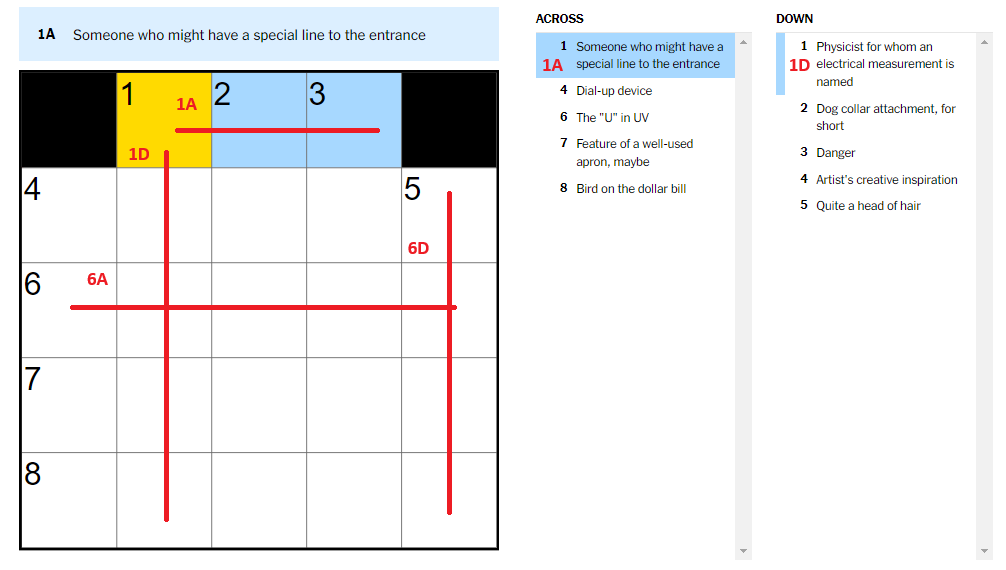
\includegraphics[width=\textwidth]{img/new-york-times-xword.png}
	\centering
	\caption{Crucigrama del New York Times}
	\label{fig:xwordNYT}
\end{figure}

\subsection{Pistas}

Un crucigrama está formado por palabras en vertical y en horizontal. Para
solucionar el crucigrama se da una serie de pistas. Estas pistas pueden
referenciarse en el crucigrama de 2 formas distintas.



\begin{itemize}
	\item La cuadrícula
	\item Las pistas
	\item El número de palabras que hay en un crucigrama es la suma de
	las palabras en horizontal y en vertical.
\end{itemize}


El modelo de datos es relativamente simple una cuadrícula que tiene celdas
en negro donde no se puede

\subsection{Algoritmo}

En esta sección describiremos brevemente el algoritmo utilizado para detectar
las etiquetas que tiene el crucigrama. Está pensado para trabajar
con los crucigramas Americanos \cite{XwordRules} que como ya he mencionado
previamente las palabras están formadas al menos por 3 letras.

A continuación se muestra el pseudocódigo \cite{pseudocode} que decribe al
algoritmo:

\begin{verbatim}
	posicionesHorizontales = {}
	posicionesVerticales = {}
	numeroEtiqueta = 0
	
	Procedimiento detectarEtiquetas(crucigrama)
	Fin Procedimiento
\end{verbatim}

\section{Conclusiones}

\section{Anexo}

\subsection{Prerequisitos}

\begin{itemize}
	\item NodeJS 20.X.X o superior (recomiendo la versión LTS)
	\item Docker Desktop (Windows), Docker (Linux)
\end{itemize}

Para arrancar tanto el frontend como el backend se necesita alguna distribución
de NodeJS instalada. Para arrancar el backend hay que seguir los siguientes pasos:

\begin{verbatim}
Antes de arrancar el back necesita que el driver de mongodb para
express se conecte a una instancia en el ordenador,
si utiliza docker:
> docker run --name xword -p 27017:27017 -d mongo:latest

Una vez arrancada la BBDD puede arrancar el backend
	
Sitúese en la capeta back
> cd back
> npm install
> npm build  # Crea una carpeta dist en el que se encontrarán
los archivos .js requeridos para ejecutar el servidor de express

Después de arrancar mongo ya está en condiciones para arrancar
el servidor de express
> node dist/index.js
\end{verbatim}

Para arrancar el frontend tiene que situarse en la carpeta front y ejecutar

\begin{verbatim}
> cd front
> npm install
> npm run dev
\end{verbatim}

\begin{thebibliography}{100}
	\bibitem{XwordRules} Shortz, W. (s.f). \textit{Real Rules of the Puzzle}.
	BarelyBad. https://barelybad.com/xwdrulesreal.htm
	\bibitem{pseudocode} Wikipedia (s.f). \textit{Pseudocódigo}. Wikipedia. https://es.wikipedia.org/wiki/Pseudoc\%C3\%B3digo
	\bibitem{OneLook} OneLook (s.f). \textit{OneLook}. https://onelook.com/

\end{thebibliography}



\end{document}